\documentclass[12pt,a4paper]{article}
\usepackage{fontspec}
\XeTeXlinebreaklocale "th"
\XeTeXlinebreakskip=0pt plus 1pt
\defaultfontfeatures{Ligatures=TeX}
\setmainfont[
  Path={fonts/TH Sarabun PSK V-1/},
  Extension=.ttf,
  UprightFont={*},
  BoldFont={* Bold},
  ItalicFont={* Italic},
  BoldItalicFont={* BoldItalic}
]{THSarabun}
\setmonofont{Latin Modern Mono}
\usepackage{amsmath,amssymb,mathtools}
\usepackage{graphicx,float,caption,xcolor}
\usepackage{geometry,booktabs,tabularx,array}
\usepackage{tikz}
\usetikzlibrary{arrows.meta,positioning,calc,shapes.geometric}
\usepackage{enumitem}
\usepackage[hidelinks]{hyperref}
\geometry{top=0.52in,bottom=0.50in,left=0.58in,right=0.58in}
\setlength{\parindent}{1.5em}
\setlength{\parskip}{0pt}
\linespread{0.95}
\emergencystretch=2em
\renewcommand{\arraystretch}{1.12}
\setlength{\tabcolsep}{4pt}
\captionsetup{font=normalsize,labelfont=bf}
\renewcommand{\figurename}{รูปที่}
\renewcommand{\tablename}{ตารางที่}
\setlist[enumerate]{leftmargin=2.2em,itemsep=0.15em,topsep=0.25em}
\setlist[itemize]{leftmargin=2.0em,itemsep=0.15em,topsep=0.25em}
\pagestyle{plain}
\definecolor{navy}{RGB}{24,54,93}
\definecolor{teal}{RGB}{0,110,112}
\definecolor{lightblue}{RGB}{238,245,250}
\definecolor{lightgreen}{RGB}{238,248,241}
\newcommand{\pu}{\ensuremath{\,\mathrm{pu}}}
\newcommand{\hz}{\ensuremath{\,\mathrm{Hz}}}
\newcommand{\second}{\ensuremath{\,\mathrm{s}}}
\newcommand{\sci}[2]{\ensuremath{#1\times10^{#2}}}
\newcommand{\templateheading}[1]{\vspace{0.42em}\noindent{\fontsize{20}{22}\selectfont\bfseries #1}\par\vspace{0.18em}}
\newcommand{\templatesubheading}[1]{\vspace{0.30em}\noindent{\fontsize{20}{22}\selectfont\bfseries #1}\par\vspace{0.12em}}
% Generated by generate_ieee14_gfm_lock_comparison. Do not edit.
% Every number the comparison section prints comes from here, so the prose cannot drift
% from the runs. Arm keys: adaptive, pinned_gfm1, pinned_gfm2, pinned_gfm4, locked_gfl

\newcommand{\ArmAdaptiveLabel}{adaptive}
\newcommand{\ArmAdaptiveHorizon}{250.000}
\newcommand{\ArmAdaptiveConverged}{1}
\newcommand{\ArmAdaptiveReclose}{159.2397}
\newcommand{\ArmAdaptiveGfmMax}{4}
\newcommand{\ArmAdaptiveFailure}{--}
\newcommand{\ArmAdaptiveSamples}{4990}
\newcommand{\ArmAdaptiveRejected}{135}
\newcommand{\DfAdaptiveSGtrip}{0.7587}
\newcommand{\SetAdaptiveSGtrip}{0.0041}
\newcommand{\DfAdaptiveLoadstep}{1.0035}
\newcommand{\SetAdaptiveLoadstep}{0.3753}
\newcommand{\DfAdaptiveFault}{1.1386}
\newcommand{\SetAdaptiveFault}{0.3753}
\newcommand{\DfAdaptiveLinetrip}{0.3764}
\newcommand{\SetAdaptiveLinetrip}{0.3503}
\newcommand{\DfAdaptiveRestorereclose}{1.1612}
\newcommand{\SetAdaptiveRestorereclose}{0.0130}
\newcommand{\ArmPinnedgfmOneLabel}{pinned 1 GFM}
\newcommand{\ArmPinnedgfmOneHorizon}{250.000}
\newcommand{\ArmPinnedgfmOneConverged}{1}
\newcommand{\ArmPinnedgfmOneReclose}{151.4244}
\newcommand{\ArmPinnedgfmOneGfmMax}{1}
\newcommand{\ArmPinnedgfmOneFailure}{--}
\newcommand{\ArmPinnedgfmOneSamples}{3232}
\newcommand{\ArmPinnedgfmOneRejected}{542}
\newcommand{\DfPinnedgfmOneSGtrip}{0.5312}
\newcommand{\SetPinnedgfmOneSGtrip}{0.0113}
\newcommand{\DfPinnedgfmOneLoadstep}{1.4478}
\newcommand{\SetPinnedgfmOneLoadstep}{1.2214}
\newcommand{\DfPinnedgfmOneFault}{1.4979}
\newcommand{\SetPinnedgfmOneFault}{1.2296}
\newcommand{\DfPinnedgfmOneLinetrip}{1.2325}
\newcommand{\SetPinnedgfmOneLinetrip}{1.1426}
\newcommand{\DfPinnedgfmOneRestorereclose}{1.1736}
\newcommand{\SetPinnedgfmOneRestorereclose}{0.0210}
\newcommand{\ArmPinnedgfmTwoLabel}{pinned 2 GFM}
\newcommand{\ArmPinnedgfmTwoHorizon}{250.000}
\newcommand{\ArmPinnedgfmTwoConverged}{1}
\newcommand{\ArmPinnedgfmTwoReclose}{149.9191}
\newcommand{\ArmPinnedgfmTwoGfmMax}{2}
\newcommand{\ArmPinnedgfmTwoFailure}{--}
\newcommand{\ArmPinnedgfmTwoSamples}{3183}
\newcommand{\ArmPinnedgfmTwoRejected}{321}
\newcommand{\DfPinnedgfmTwoSGtrip}{0.3489}
\newcommand{\SetPinnedgfmTwoSGtrip}{0.0001}
\newcommand{\DfPinnedgfmTwoLoadstep}{0.7839}
\newcommand{\SetPinnedgfmTwoLoadstep}{0.7123}
\newcommand{\DfPinnedgfmTwoFault}{0.8255}
\newcommand{\SetPinnedgfmTwoFault}{0.7126}
\newcommand{\DfPinnedgfmTwoLinetrip}{0.7135}
\newcommand{\SetPinnedgfmTwoLinetrip}{0.6422}
\newcommand{\DfPinnedgfmTwoRestorereclose}{0.6634}
\newcommand{\SetPinnedgfmTwoRestorereclose}{0.0209}
\newcommand{\ArmPinnedgfmFourLabel}{pinned 4 GFM}
\newcommand{\ArmPinnedgfmFourHorizon}{25.491}
\newcommand{\ArmPinnedgfmFourConverged}{0}
\newcommand{\ArmPinnedgfmFourReclose}{--}
\newcommand{\ArmPinnedgfmFourGfmMax}{4}
\newcommand{\ArmPinnedgfmFourFailure}{\texttt{adaptiveDtMin}}
\newcommand{\ArmPinnedgfmFourSamples}{819}
\newcommand{\ArmPinnedgfmFourRejected}{449}
\newcommand{\DfPinnedgfmFourSGtrip}{0.9898}
\newcommand{\SetPinnedgfmFourSGtrip}{--}
\newcommand{\DfPinnedgfmFourLoadstep}{--}
\newcommand{\SetPinnedgfmFourLoadstep}{--}
\newcommand{\DfPinnedgfmFourFault}{--}
\newcommand{\SetPinnedgfmFourFault}{--}
\newcommand{\DfPinnedgfmFourLinetrip}{--}
\newcommand{\SetPinnedgfmFourLinetrip}{--}
\newcommand{\DfPinnedgfmFourRestorereclose}{--}
\newcommand{\SetPinnedgfmFourRestorereclose}{--}
\newcommand{\ArmLockedgflLabel}{locked GFL}
\newcommand{\ArmLockedgflHorizon}{20.000}
\newcommand{\ArmLockedgflConverged}{0}
\newcommand{\ArmLockedgflReclose}{--}
\newcommand{\ArmLockedgflGfmMax}{0}
\newcommand{\ArmLockedgflFailure}{\texttt{noVoltageFormingSource}}
\newcommand{\ArmLockedgflSamples}{43}
\newcommand{\ArmLockedgflRejected}{0}
\newcommand{\DfLockedgflSGtrip}{--}
\newcommand{\SetLockedgflSGtrip}{--}
\newcommand{\DfLockedgflLoadstep}{--}
\newcommand{\SetLockedgflLoadstep}{--}
\newcommand{\DfLockedgflFault}{--}
\newcommand{\SetLockedgflFault}{--}
\newcommand{\DfLockedgflLinetrip}{--}
\newcommand{\SetLockedgflLinetrip}{--}
\newcommand{\DfLockedgflRestorereclose}{--}
\newcommand{\SetLockedgflRestorereclose}{--}
\newcommand{\CommonWindowPinnedgfmOneBitIdentical}{1}
\newcommand{\CommonWindowPinnedgfmOneSamples}{42}
\newcommand{\CommonWindowPinnedgfmTwoBitIdentical}{1}
\newcommand{\CommonWindowPinnedgfmTwoSamples}{42}
\newcommand{\CommonWindowPinnedgfmFourBitIdentical}{1}
\newcommand{\CommonWindowPinnedgfmFourSamples}{42}
\newcommand{\CommonWindowLockedgflBitIdentical}{1}
\newcommand{\CommonWindowLockedgflSamples}{42}
\newcommand{\CommonWindowSplit}{20.000}
\newcommand{\CommonWindowAllBitIdentical}{1}
\newcommand{\CandTotal}{15}
\newcommand{\CandReady}{7}
\newcommand{\CandBestSet}{IBR3+IBR6}
\newcommand{\CandBestN}{2}
\newcommand{\CandBestOmega}{-0.56814}
\newcommand{\CandBestSingleOmega}{-0.32801}
\newcommand{\CandFullOmega}{-0.48291}
\newcommand{\CandReadyNOne}{4}
\newcommand{\CandTotalNOne}{4}
\newcommand{\CandReadyNTwo}{2}
\newcommand{\CandTotalNTwo}{6}
\newcommand{\CandReadyNThree}{0}
\newcommand{\CandTotalNThree}{4}
\newcommand{\CandReadyNFour}{1}
\newcommand{\CandTotalNFour}{1}

% Generated by generate_ieee14_report_scalars. Do not edit.
%
% PROVENANCE. Accepted values of output/diagnostics/ieee14_gfm_lock_compare_dcreal/adaptive_250s.mat.
% Produced by run_ieee14_gfm_lock_comparison, whose option set is the
% flagship driver's plus agsi_reference=true (opt-in, post-processing only).
% This cache is NOT bit-identical to the earlier delivered artifact, and no
% such claim is made for it: the DC-link closure changed under
% NUM-2026-08-20-01, so the trajectory legitimately differs. Compare it to
% the earlier cache by outcome, never by bit-identity.
% No value here is rounded, scaled, smoothed or otherwise altered.
%
% Regenerate with:  pf_init_paths; generate_ieee14_report_scalars(result_file="output/diagnostics/ieee14_gfm_lock_compare_dcreal/adaptive_250s.mat")

\newcommand{\NewRunEnd}{250.000}
\newcommand{\NewRunVMin}{0.036855}
\newcommand{\NewRunVMax}{1.523183}
\newcommand{\NewRunFMin}{58.838795}
\newcommand{\NewRunFMax}{61.138560}
\newcommand{\NewRunSubdivision}{0}
\newcommand{\NewRunDomainRejects}{584}
\newcommand{\NewRunResidual}{$9.9596\times10^{-9}$}
\newcommand{\NewRunReclose}{159.240}
\newcommand{\NewRunRecloseStatus}{SUCCESS}
\newcommand{\NewRunSyncDV}{0.008785}
\newcommand{\NewRunSyncDF}{$6.4601\times10^{-13}$}
\newcommand{\NewRunSyncDTheta}{5.015017}
\newcommand{\NewRunFirstRelease}{25.310}
\newcommand{\NewRunReleaseOne}{25.310}
\newcommand{\NewRunReleaseTwo}{146.247}
\newcommand{\NewRunReleaseThree}{152.390}
\newcommand{\NewRunReleaseFour}{--}
\newcommand{\NewRunAugmentOne}{22.052}
\newcommand{\NewRunAugmentTwo}{51.333}
\newcommand{\NewRunAugmentThree}{53.372}
\newcommand{\NewRunAugmentFour}{148.267}
\newcommand{\NewRunNRelease}{3}
\newcommand{\NewRunNAugment}{4}
\newcommand{\NewRunGfmMax}{4}
\newcommand{\NewRunSamples}{4990}
\newcommand{\NewRunRejectedSteps}{135}
\newcommand{\NewRunTerminalF}{60.000000}
\newcommand{\NewRunTerminalVMin}{0.9667}
\newcommand{\NewRunTerminalVMax}{1.0575}
\newcommand{\NewRunStepper}{adaptive}
\newcommand{\NewRunReselection}{NO\_FEASIBLE\_SG\_ON\_ONE\_STEP}

\graphicspath{{figures/}{figures/final_report_th/}{figures/presentation_pf_sssa_ts_gfm/}}

\begin{document}
\makeatletter
\renewcommand\normalsize{\@setfontsize\normalsize{18}{19.5}}
\makeatother
\normalsize
\begin{titlepage}
\thispagestyle{empty}
\begin{center}
\vspace*{0.20in}
{\fontsize{26}{31}\selectfont\bfseries เอกสารสรุปวิชาโครงงาน\par}
\vspace{0.32in}
{\fontsize{18}{22}\selectfont\bfseries ชื่องานโครงงาน\par}
\vspace{0.12in}
{\fontsize{19}{24}\selectfont\bfseries
(ภาษาไทย) กรอบการสลับโหมดแบบอัตโนมัติระหว่าง Grid-Following และ Grid-Forming\\
สำหรับทรัพยากรที่เชื่อมต่อผ่านอินเวอร์เตอร์\par}
\vspace{0.13in}
{\fontsize{18}{22}\selectfont\bfseries
(ภาษาอังกฤษ) An Automatic Following/Forming Framework\\
for Inverter-Based Resources\par}
\vspace{0.38in}
{\fontsize{18}{22}\selectfont\bfseries สมาชิกผู้จัดทำ\par}
\vspace{0.08in}
{\fontsize{18}{22}\selectfont
1. Phichitchai Jueajan \hspace{0.35in} 66010569\\
2. Pakkapol Phdungdan \hspace{0.35in} 66010612\par}
\vspace{0.28in}
{\fontsize{18}{22}\selectfont\bfseries อาจารย์ที่ปรึกษา\par}
\vspace{0.08in}
{\fontsize{18}{22}\selectfont
1. Dr. Tossaporn Surinkaew\\
2. Prof. Dr. Issarachai Ngamroo\par}
\vfill
{\fontsize{18}{22}\selectfont
ภาควิชาวิศวกรรมไฟฟ้า คณะวิศวกรรมศาสตร์\\
สถาบันเทคโนโลยีพระจอมเกล้าเจ้าคุณทหารลาดกระบัง\par}
\vspace{0.15in}
{\fontsize{18}{22}\selectfont\bfseries ปีการศึกษา 2569\par}
\end{center}
\end{titlepage}
\templateheading{วัตถุประสงค์ของโครงงาน}
\begin{enumerate}
\item ศึกษาและพัฒนาสายงานคำนวณระบบไฟฟ้ากำลังที่เชื่อมโยงการไหลของกำลัง (Power Flow: PF) การวิเคราะห์เสถียรภาพสัญญาณขนาดเล็ก (Small-Signal Stability Analysis: SSSA) และการจำลองโดเมนเวลา (Time-Domain Simulation: TS) ภายใต้แบบจำลองเดียวกัน
\item พัฒนาแบบจำลองทรัพยากรที่เชื่อมต่อผ่านอินเวอร์เตอร์ (Inverter-Based Resources: IBR) ที่สามารถทำงานได้ทั้งโหมด Grid-Following (GFL) และ Grid-Forming (GFM)
\item พัฒนากลไก supervisor สำหรับสลับโหมด GFL/GFM อัตโนมัติตามสภาวะของระบบ โดยรักษาความต่อเนื่องของ state และกระแสที่จุดเชื่อมต่อ
\item ทดสอบกรอบการทำงานบนระบบ IEEE 14-bus ภายใต้เหตุการณ์รบกวนหลายชนิด และเปรียบเทียบผลกับนโยบายการควบคุมแบบอื่น
\end{enumerate}

\clearpage
\templateheading{ความสำคัญ และที่มาของปัญหาที่ทำโครงงาน}
ระบบไฟฟ้ากำลังในปัจจุบันมีสัดส่วนแหล่งพลังงานที่เชื่อมต่อผ่านอินเวอร์เตอร์เพิ่มขึ้นอย่างต่อเนื่อง เช่น ระบบผลิตไฟฟ้าจากพลังงานหมุนเวียนและระบบกักเก็บพลังงาน อุปกรณ์เหล่านี้มีพฤติกรรมแตกต่างจากเครื่องกำเนิดไฟฟ้าซิงโครนัส (Synchronous Generator: SG) ซึ่งเดิมเป็นแหล่งกำหนดแรงดัน ความถี่ และมุมอ้างอิงให้กับโครงข่าย

IBR แบบ GFL ทำงานโดยอาศัยแรงดันของโครงข่ายเป็นสัญญาณอ้างอิงผ่านวงจร Phase-Locked Loop (PLL) จึงเหมาะกับระบบที่มีแหล่งสร้างกริดอยู่แล้ว ในทางตรงกันข้าม GFM สามารถสร้างมุมและแรงดันอ้างอิงของตนเองได้ และจึงมีบทบาทสำคัญเมื่อระบบสูญเสีย SG หรือเข้าสู่สภาวะกริดอ่อน อย่างไรก็ตาม การกำหนดให้ IBR ทุกตัวทำงานเป็น GFM ตลอดเวลาไม่จำเป็นต้องให้ผลดีที่สุด และอาจเพิ่มความซับซ้อนของการควบคุมหรือทำให้การจำลองไม่ผ่านในบางสภาวะ
โครงงานนี้จึงเสนอกรอบการทำงานที่ให้ IBR เปลี่ยนบทบาทระหว่าง GFL และ GFM ตามความจำเป็นของระบบ โดยใช้ผลจาก PF, equilibrium, SSSA และสถานะที่ยอมรับแล้วจาก TS เป็นพื้นฐานในการตัดสินใจ การทดสอบหลักใช้ระบบ IEEE 14-bus ซึ่งประกอบด้วย SG ที่บัส 1 และ IBR จำนวน 4 ตัวที่บัส 2, 3, 6 และ 8 ดังรูปที่~\ref{fig:network}

\begin{figure}[H]
\centering
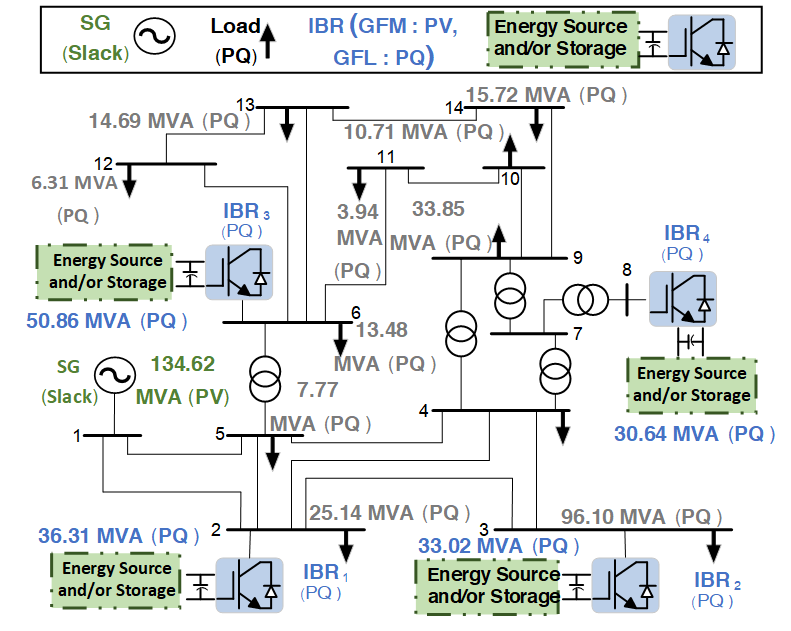
\includegraphics[width=0.64\textwidth]{123313.png}
\caption{ระบบ IEEE 14-bus ที่ใช้เป็นกรณีศึกษา โดยมี SG และ IBR แบบ GFL/GFM}
\label{fig:network}
\end{figure}

กรณีศึกษาถูกออกแบบให้เกิดการสูญเสีย SG การเปลี่ยนโหลด fault การปลดสายส่ง และการคืน SG เพื่อให้เห็นความจำเป็นของการเปลี่ยนบทบาทของ IBR อย่างชัดเจน หากไม่มีแหล่ง voltage-forming หลัง SG ถูกปลด ระบบจะไม่มีผู้ถือมุมอ้างอิงและตัวแก้สมการจะต้องหยุดแบบ fail-closed แทนการบังคับให้ผลลัพธ์ผ่าน

\clearpage
\templateheading{การดำเนินงานและผลงานที่ได้รับจากโครงงาน (โดยสังเขป) พร้อมภาพประกอบ}
\templatesubheading{1. โครงสร้างระบบศึกษาและสายงาน PF--DAE--SSSA--TS}
โครงงานพัฒนาสายงานคำนวณแบบต่อเนื่องโดยใช้ข้อมูลเครือข่าย จุดทำงาน และแบบจำลองอุปกรณ์ชุดเดียวกันตลอดทั้ง Power Flow (PF), การหาจุดสมดุลของ Differential-Algebraic Equations (DAE), Small-Signal Stability Analysis (SSSA) และ Time-Domain Simulation (TS) จุดประสงค์สำคัญคือไม่ให้แต่ละขั้นตอนใช้สมมติฐานหรือ state ที่ไม่ตรงกัน จึงสามารถย้อนตรวจได้ว่าผล SSSA และ TS เริ่มจาก operating point เดียวกับ PF จริง
\begin{equation}
\dot{x}=f(x,y,u),\qquad 0=g(x,y,u)=Y_{\mathrm{net}}V-I_{\mathrm{bus}}(x,V)
\label{eq:dae_summary}
\end{equation}
โดย $x$ คือ differential states ของ SG และ IBR, $y$ คือ algebraic bus voltages ในรูปส่วนจริงและส่วนจินตภาพ, $u$ คือ set-point และข้อมูล event ส่วน $Y_{\mathrm{net}}$ สร้างจากข้อมูลสายส่ง หม้อแปลง และ shunt ของ IEEE 14-bus ทั้งหมด การคำนวณทุกขั้นใช้ convention เดียวกันคือกระแสบวกหมายถึงฉีดเข้าสู่โครงข่าย และกำลังเชิงซ้อน $S=V I^{*}$

\begin{figure}[H]
\centering
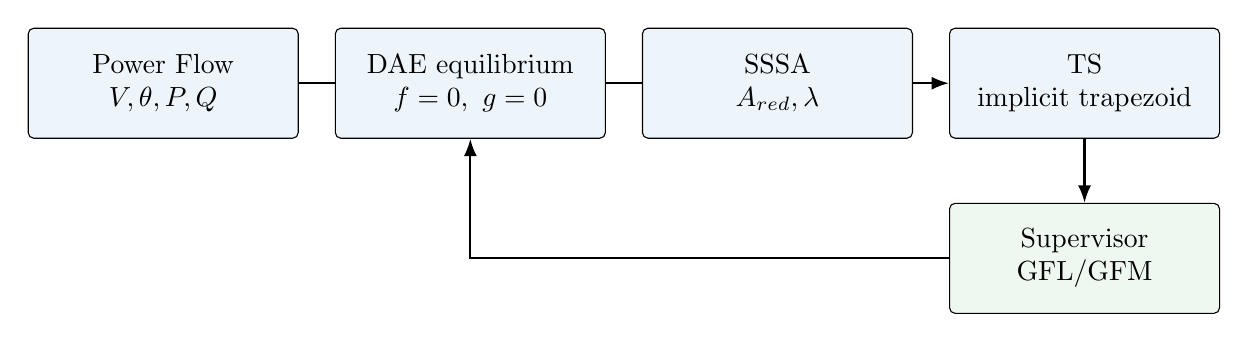
\begin{tikzpicture}[
  box/.style={draw=black,rounded corners=2pt,minimum width=1.35in,minimum height=0.55in,align=center,fill=lightblue},
  arr/.style={-{Latex[length=2.2mm]},thick}]
\node[box] (pf) {Power Flow\\$V,\theta,P,Q$};
\node[box,right=0.18in of pf] (eq) {DAE equilibrium\\$f=0,\ g=0$};
\node[box,right=0.18in of eq] (sssa) {SSSA\\$A_{red},\lambda$};
\node[box,right=0.18in of sssa] (ts) {TS\\implicit trapezoid};
\node[box,below=0.32in of ts,fill=lightgreen] (sup) {Supervisor\\GFL/GFM};
\draw[arr] (pf)--(eq)--(sssa)--(ts);
\draw[arr] (ts)--(sup);
\draw[arr] (sup.west) -| (eq.south);
\end{tikzpicture}
\caption{สายงานคำนวณหลักของโครงงาน ตั้งแต่ PF ถึงการสลับโหมดใน TS}
\label{fig:pipeline}
\end{figure}

\templatesubheading{2. Power Flow และการสร้าง operating point ของ IEEE 14-bus}
Power Flow ใช้สำหรับหาขนาดแรงดันและมุมของทุกบัสก่อนเริ่มการวิเคราะห์เชิงพลวัต สำหรับบัส $i$ กำลังสุทธิที่ฉีดเข้าโครงข่ายเขียนได้เป็น
\begin{equation}
P_i+jQ_i=V_i\left(\sum_{j=1}^{N}Y_{ij}V_j\right)^{*}.
\label{eq:pfpower}
\end{equation}
บัสถูกแบ่งเป็น REF, PV และ PQ ตามตัวแปรที่กำหนดและตัวแปรที่ต้องแก้ โดยบัส REF กำหนด $|V|$ และ $\theta$, บัส PV กำหนด $P$ และ $|V|$, ส่วนบัส PQ กำหนด $P$ และ $Q$. ตัวแก้ Newton--Raphson สร้าง mismatch $\Delta P,\Delta Q$ แล้วแก้ระบบเชิงเส้น
\begin{equation}
\begin{bmatrix}\Delta P\\ \Delta Q\end{bmatrix}=
\begin{bmatrix}J_{P\theta}&J_{PV}\\J_{Q\theta}&J_{QV}\end{bmatrix}
\begin{bmatrix}\Delta\theta\\\Delta |V|\end{bmatrix},
\label{eq:pfnewton}
\end{equation}
ทำซ้ำจน mismatch อยู่ใน tolerance ที่กำหนด จากนั้นผลแรงดันเชิงซ้อน $V_i=|V_i|e^{j\theta_i}$ จะถูกส่งต่อให้ตัวสร้าง state ของ SG และ IBR โดยตรง ไม่สร้าง operating point ชุดใหม่สำหรับ SSSA หรือ TS

ผล PF ล่าสุดของกรณี SG-online ซึ่งเป็นชุดผลเดียวกับรายงาน IEEE 14-bus ที่อาจารย์ตรวจแล้ว แสดงค่าหลักดังตารางที่~\ref{tab:pf_key}. SG ที่บัส 1 เป็น reference source ในช่วงเริ่มต้น และ IBR อยู่ที่บัส 2, 3, 6 และ 8
\begin{table}[H]
\centering
\caption{ค่าหลักจาก Power Flow ของ IEEE 14-bus ก่อนเกิด disturbance}
\label{tab:pf_key}
\begin{tabularx}{0.96\textwidth}{@{}r l r r r r@{}}
\toprule
Bus & Type & $|V|$ (pu) & $\theta$ (deg) & $P_g$ (pu) & $Q_g$ (pu) \\
\midrule
1 & REF & 1.0000 & 0.0000 & 1.3319 & -0.1957 \\
2 & GFL & 0.9914 & -3.2585 & 0.3172 & 0.1767 \\
3 & GFL & 0.9667 & -8.6921 & 0.2884 & 0.1607 \\
6 & GFL & 1.0575 & -6.7136 & 0.4443 & 0.2476 \\
8 & GFL & 1.0494 & -4.4090 & 0.2677 & 0.1491 \\
\bottomrule
\end{tabularx}
\end{table}
การตรวจสอบ PF ไม่ได้ดูเฉพาะการที่ Newton รายงานว่า converged แต่ตรวจ power balance, branch flow/loss และค่ากระแสที่คำนวณกลับจาก $S=VI^{*}$. จากนั้นเมื่อแปลง PF ไปเป็น DAE equilibrium จะคง KCL ของทุกบัสไว้ครบ ไม่ตัด KCL ของบัส reference ออกเพื่อทำให้สมการเป็นสี่เหลี่ยม แต่ใช้การ fix พิกัด reference และแก้ control input ที่เหมาะสมแทน วิธีนี้ป้องกันกรณีที่ reduced residual เล็กแต่ physical KCL ยังผิด

\templatesubheading{3. DAE equilibrium และแบบจำลอง Synchronous Generator}
หลัง PF ได้แรงดันและกำลังของแต่ละอุปกรณ์ จะสร้าง state เริ่มต้นและแก้สมการ $f=0$ ร่วมกับ KCL $g=0$ อีกครั้ง จุดสมดุลนี้เป็นจุดเริ่มต้นร่วมของ SSSA และ TS สำหรับ SG ที่บัส 1 ใช้แบบจำลอง round-rotor sixth-order โดย state ที่เก็บคือ
\begin{equation}
x_{SG}=[\delta,\omega,E'_q,E'_d,E''_q,E''_d]^T,
\end{equation}
และแกนกลใช้ swing equation
\begin{equation}
\dot{\delta}=\omega_0\Delta\omega,\qquad
2H\dot{\Delta\omega}=T_m-T_e-D\Delta\omega.
\label{eq:swing_summary}
\end{equation}
ส่วน transient/subtransient EMF ใช้ time constants และ reactances ของโปรไฟล์ IEEE 14-bus ในโปรเจกต์ กรณีนี้ $T'_{q0}=0$ จึงเป็น singular limit และ state $E'_d$ ถูกตรึงที่ค่าพีชคณิตก่อน equilibrium/SSSA ทำให้ SG มี active dynamic states จริง 5 ตัว ไม่ใช่การเพิ่ม time constant เล็ก ๆ เพื่อหลบ singularity

เมื่อ SG breaker เปิด SG จะหยุดฉีดกระแสเข้าระบบ แต่ state ทางกลและ flux ยังถูก integrate ต่อในเส้นทาง breaker-open coast จึงสามารถตรวจ synchronism ก่อน reclose ได้ โดยไม่ reset มุมหรือความเร็วของ SG ให้เท่ากับบัสแบบบังคับ
\clearpage
\templatesubheading{4. Small-Signal Stability Analysis (SSSA)}
SSSA ใช้ตรวจพฤติกรรมของระบบเมื่อถูกรบกวนขนาดเล็กรอบจุดสมดุล โดย linearize สมการ DAE ชุดเดียวกับที่ใช้ใน TS
\begin{equation}
\begin{bmatrix}\Delta\dot{x}\\0\end{bmatrix}=
\begin{bmatrix}f_x&f_y\\g_x&g_y\end{bmatrix}
\begin{bmatrix}\Delta x\\\Delta y\end{bmatrix}.
\label{eq:sssa_full}
\end{equation}
เมื่อ $g_y$ ไม่เอกฐาน สามารถกำจัด algebraic perturbation ด้วย Schur complement ได้
\begin{equation}
A_{\mathrm{red}}=f_x-f_y g_y^{-1}g_x,
\qquad \Delta\dot{x}=A_{\mathrm{red}}\Delta x.
\label{eq:sssa_schur}
\end{equation}
Eigenvalue $\lambda=\sigma\pm j\omega_d$ ใช้บอกอัตราการสลายและการสั่นของ mode โดย
\begin{equation}
f_m=\frac{|\omega_d|}{2\pi},\qquad
\zeta=-\frac{\sigma}{\sqrt{\sigma^2+\omega_d^2}}.
\label{eq:modalmetrics}
\end{equation}
หาก eigenvalue ที่เป็น physical decision roots ทั้งหมดมี real part เป็นลบ ระบบที่จุดนั้นมี small-signal stability อย่างไรก็ตาม SSSA เป็นเพียง local linear result จึงไม่ใช้แทน nonlinear TS

การจัดการ reference angle เป็นส่วนสำคัญของ SSSA เนื่องจากระบบมี freedom ของมุมร่วมหนึ่งค่า โครงงานจัดการ gauge ก่อนคำนวณ eigenvalue ด้วย active-state/reference-coordinate projection ที่สอดคล้องกับ configuration จริง ไม่ใช้วิธีคำนวณ eigenvalue ก่อนแล้วค่อยลบ zero root ภายหลัง และยังเก็บ physical KCL ทุกแถวไว้ครบ วิธีนี้ทำให้จำนวน root ที่ใช้ตัดสินใจสอดคล้องกับ degree of freedom ที่แท้จริงของระบบ

สำหรับ configuration ตัวแทนหลัง SG offline ที่ IBR2 เป็น GFM และ IBR3/6/8 เป็น GFL spectrum อยู่ใน left-half plane ทั้งหมด mode ขวาสุดคือ
\begin{equation}
\lambda=-0.328014\pm j0.448860\ \mathrm{s}^{-1},
\quad f=0.071438\ \mathrm{Hz},\quad \zeta=0.590017.
\end{equation}
ในกลุ่ม PLL mode พบคู่ $-0.566771\pm j2.132137$ s$^{-1}$ ที่ $f=0.33934$ Hz และ $\zeta=0.256901$. ส่วน DC-link ของ IBR ทั้งสี่ให้คู่ mode ใกล้ $15.18$--$15.66$ Hz และ $\zeta\approx0.707$ ซึ่งตรงกับ damping target ของวงจร DC ที่กำหนดก่อนคำนวณ spectrum จึงใช้เป็น consistency check ของแบบจำลองได้

\begin{figure}[H]
\centering
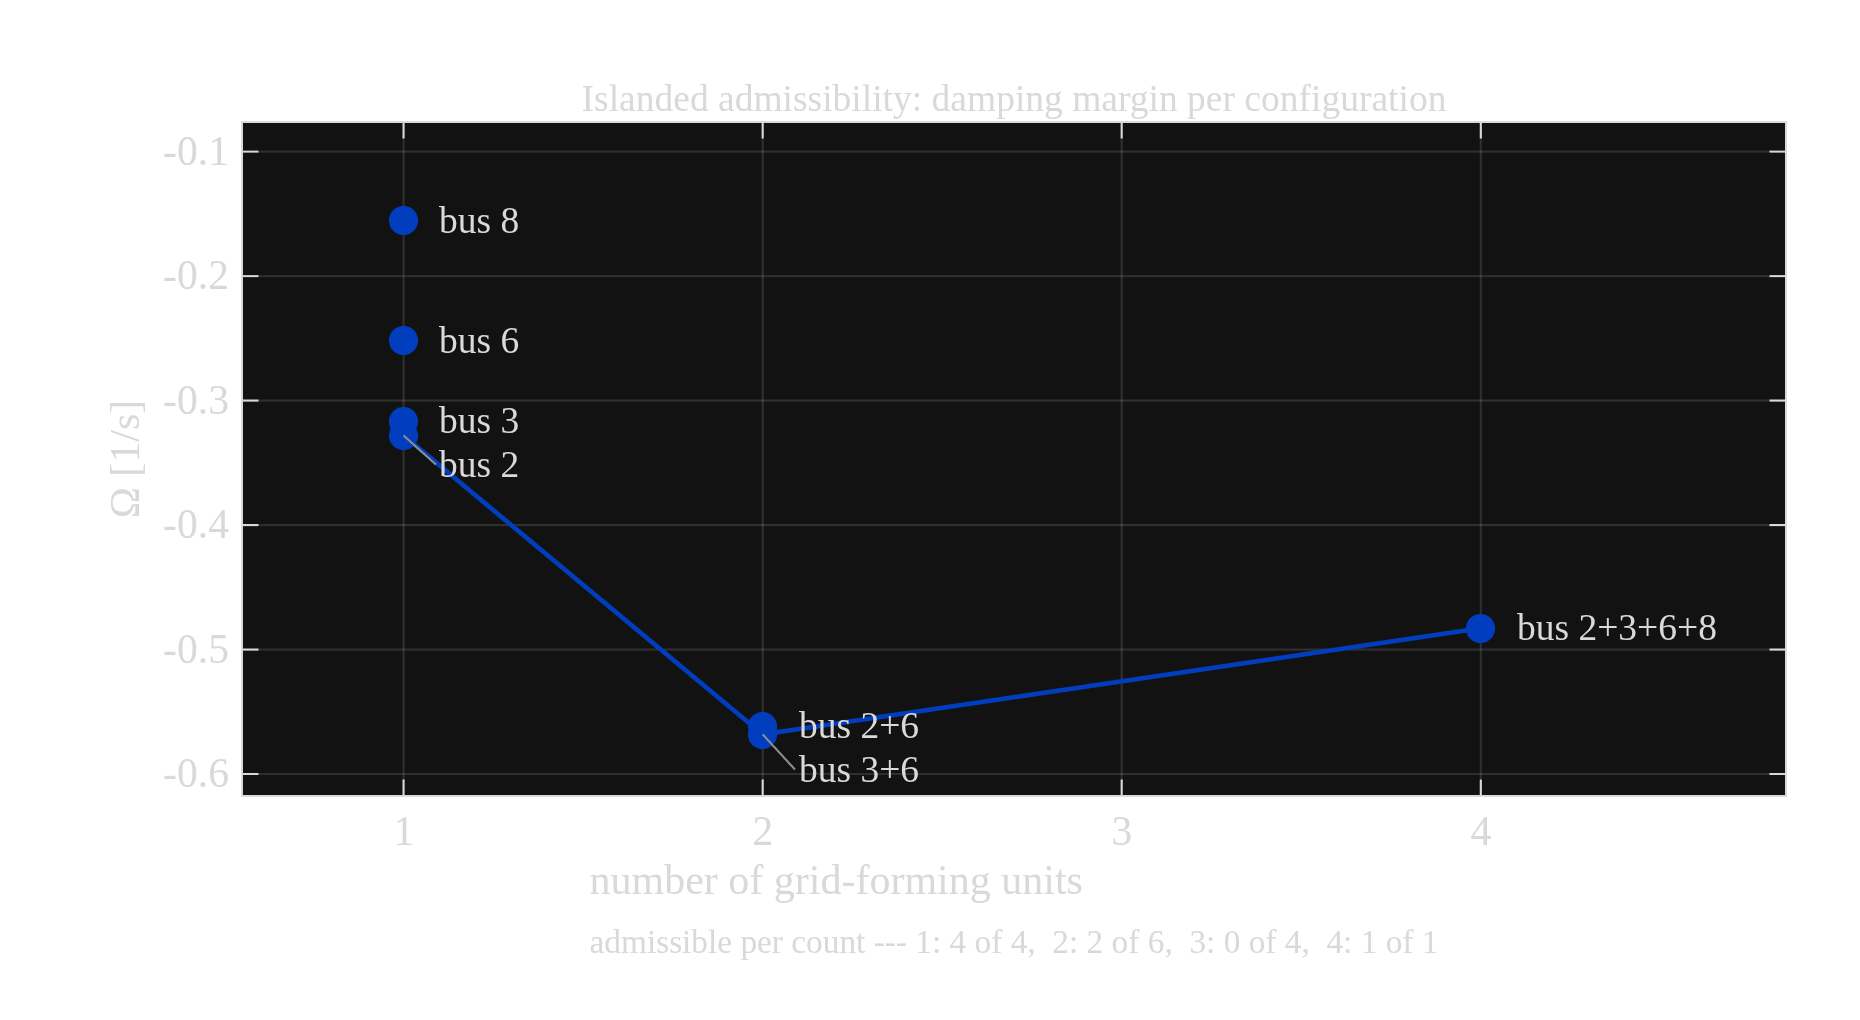
\includegraphics[width=0.88\textwidth]{switch_ieee14_decision/sg_off_admissibility.png}
\caption{Damping margin ของ candidate GFM ที่ผ่าน equilibrium และ SSSA เมื่อ SG offline บน IEEE 14-bus}
\label{fig:sssa_sweep}
\end{figure}

เมื่อ SG offline มี subset ของ IBR ที่เป็นไปได้ทั้งหมด $2^4-1=15$ candidates ระบบจะแก้ equilibrium และ SSSA ของแต่ละ candidate จาก network จริงของชุดนั้น ไม่ประมาณจากจำนวน GFM อย่างเดียว ผลล่าสุดผ่านเกณฑ์ 7 จาก 15 ชุด โดยชุดที่ให้ damping margin ดีที่สุดคือ IBR3+IBR6 จำนวน 2 ตัว มี $\Omega=-0.56814$ s$^{-1}$ ขณะที่การให้ทั้ง 4 ตัวเป็น GFM มี $\Omega=-0.48291$ s$^{-1}$. ดังนั้นจำนวน GFM ที่มากขึ้นไม่ได้ทำให้ small-signal margin ดีขึ้นแบบ monotonic

\begin{table}[H]
\centering
\caption{สรุปการคัดกรองจำนวน GFM เมื่อ SG offline}
\begin{tabularx}{0.90\textwidth}{@{}c c c X@{}}
\toprule
จำนวน GFM & จำนวน candidate & ผ่าน & ข้อสังเกต \\
\midrule
1 & 4 & 4 & ทุก single-GFM configuration ผ่าน linear screen \\
2 & 6 & 2 & ชุด IBR2+IBR6 และ IBR3+IBR6 ผ่าน; ชุดหลังให้ margin ดีที่สุด \\
3 & 4 & 0 & equilibrium ไม่ลู่เข้าภายใต้ข้อกำหนดของอุปกรณ์ \\
4 & 1 & 1 & ผ่าน SSSA แต่ต้องทดสอบ nonlinear reachability ต่อ \\
\bottomrule
\end{tabularx}
\end{table}

\templatesubheading{5. Time-Domain Simulation (TS) และ numerical solver}
TS ใช้สมการ DAE เดียวกับ~\eqref{eq:dae_summary} แล้ว discretize differential states ด้วย implicit trapezoidal method
\begin{equation}
\begin{aligned}
x_{k+1}-x_k-\frac{h}{2}\bigl[f(x_k,y_k,u_k)&+f(x_{k+1},y_{k+1},u_{k+1})\bigr]=0,\\
g(x_{k+1},y_{k+1},u_{k+1})&=0.
\end{aligned}
\label{eq:trap_summary}
\end{equation}
Unknown ของแต่ละ step จึงประกอบด้วย differential และ algebraic variables พร้อมกัน ตัวแก้ใช้ damped Newton
\begin{equation}
J(z^{(m)})\Delta z=-r(z^{(m)}),\qquad
z^{(m+1)}=z^{(m)}+\alpha\Delta z,\quad 0<\alpha\le1,
\end{equation}
และรับ step เมื่อ nonlinear residual ผ่าน gate ที่กำหนด สำหรับผลหลักทุก accepted step มี $\|r\|_{\infty}<10^{-8}$

เส้นทาง adaptive ใช้แนวคิด step-doubling ของ trapezoidal method: ทดลองหนึ่ง full step และสอง half steps แล้วประเมิน local error จากความต่างของคำตอบลำดับสอง
\begin{equation}
e_{LTE}\approx\frac{z_{h/2,h/2}-z_h}{2^2-1}=\frac{z_{h/2,h/2}-z_h}{3}.
\label{eq:lte_summary}
\end{equation}
หาก Newton ไม่ลู่เข้า, state ออกนอก physical domain หรือ LTE สูงเกินเกณฑ์ step จะถูก reject และ rollback ไปยัง accepted state เดิมก่อนลด $h$ ใหม่ จึงไม่มี rejected trial ปะปนใน trajectory ที่นำไป plot

อีกจุดหนึ่งที่สำคัญคือ exact event landing: เมื่อมี SG trip, load step, fault, fault clearing, line trip หรือ mode switching ตัว integrator จะตัด step ให้ปลาย step ตรงกับเวลา event ก่อน จากนั้นจึงเปลี่ยน topology/mode และแก้ algebraic right-limit ใหม่ วิธีนี้ป้องกันการใช้สมการก่อนและหลัง event อยู่ใน trapezoidal step เดียวกัน

การทดสอบ regression ของเส้นทาง solver แยกชัดระหว่าง fixed และ adaptive mode โดยกรณี IEEE 14-bus ที่ไม่ได้เปิด adaptive option ให้ผลเหมือนการระบุ \texttt{stepper=fixed} แบบ bit-identical สำหรับ $t$, $x$, $y$, input history และ event log ทำให้การเพิ่ม adaptive controller ไม่เปลี่ยนผลของเส้นทางเดิมโดยไม่ตั้งใจ
\clearpage
\templatesubheading{6. แบบจำลอง IBR แบบสองโหมด GFL/GFM}
IBR ที่ใช้ในกรณีหลักเป็นแบบจำลอง source-mapped จากโครงสร้าง EECON49 แล้วจัดให้อยู่ใน fixed-layout device เดียว เพื่อให้เปลี่ยนโหมดระหว่าง GFL และ GFM ได้โดยไม่เปลี่ยนขนาด state vector กลางการจำลอง แต่ละ IBR มี 17 coordinates
\begin{equation}
\begin{aligned}
x_{IBR}=[&i_d,i_q,V_{dc},\;\delta_{PLL},\xi_{PLL},\xi_P,\xi_Q,\xi_{Id}^{GFL},\xi_{Iq}^{GFL},\\
&\delta_{VSG},\omega_{VSG},E,\xi_{Vd},\xi_{Vq},\xi_{Id}^{GFM},\xi_{Iq}^{GFM},I_{dc}]^T.
\end{aligned}
\label{eq:ibr17}
\end{equation}
โหมด GFL ใช้ active states $\{1{:}9,17\}$ รวม 10 ตัว ส่วน GFM ใช้ $\{1{:}3,10{:}16,17\}$ รวม 11 ตัว state ของ branch ที่ไม่ได้ใช้งานจะถูก hold แบบ $\dot x=0$ ไม่สร้าง artificial decay pole เพื่อดึง state กลับเอง

\begin{figure}[H]
\centering
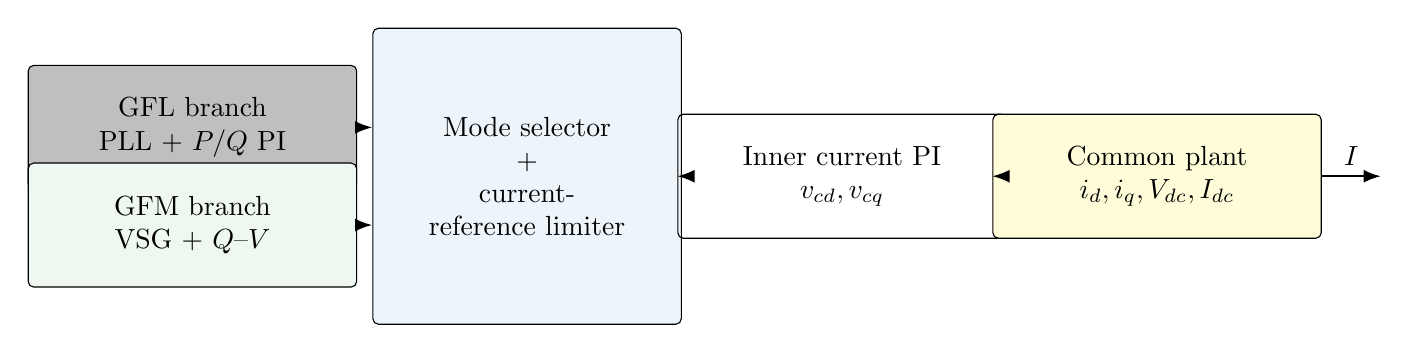
\begin{tikzpicture}[
  blk/.style={draw,rounded corners=2pt,align=center,minimum height=0.62in,text width=1.55in},
  sel/.style={draw,rounded corners=2pt,align=center,minimum height=1.48in,text width=1.45in,fill=lightblue},
  arr/.style={-{Latex[length=2.2mm]},thick}]
\node[blk,fill=lightgray] (gfl) at (0,0.62) {GFL branch\\PLL + $P/Q$ PI};
\node[blk,fill=lightgreen] (gfm) at (0,-0.62) {GFM branch\\VSG + $Q$--$V$};
\node[sel] (mode) at (4.25,0) {Mode selector\\+\\current-reference limiter};
\node[blk] (inner) at (8.25,0) {Inner current PI\\$v_{cd},v_{cq}$};
\node[blk,fill=yellow!15] (plant) at (12.25,0) {Common plant\\$i_d,i_q,V_{dc},I_{dc}$};
\draw[arr] (gfl.east)--(mode.west |- gfl.east);
\draw[arr] (gfm.east)--(mode.west |- gfm.east);
\draw[arr] (mode.east)--(inner.west);
\draw[arr] (inner.east)--(plant.west);
\draw[arr] (plant.east)--++(0.75,0) node[midway,above]{$I$};
\end{tikzpicture}
\caption{โครงสร้าง IBR แบบ dual-mode: GFL และ GFM ใช้ controller คนละ branch แต่ใช้ AC/DC plant ร่วมกัน}
\label{fig:dualibr}
\end{figure}

\noindent\textbf{Common AC filter.} ทั้งสองโหมดใช้กระแส filter และ DC link ร่วมกัน โดยใน synchronous $dq$ frame
\begin{align}
\dot i_d&=\frac{\omega_b}{L_f}\left(v_{cd}-v_d-R_fi_d+\omega_{pu}L_fi_q\right),\\
\dot i_q&=\frac{\omega_b}{L_f}\left(v_{cq}-v_q-R_fi_q-\omega_{pu}L_fi_d\right).
\label{eq:filter_dq}
\end{align}
กระแส physical $i_d,i_q$ เป็น differential states จริง ตัว current limiter จำกัด current reference ที่ controller สั่ง ไม่ได้ clip state ของ filter แบบพีชคณิต เพราะการ clip state จะเปลี่ยน terminal KCL โดยตรง

\noindent\textbf{DC-link และแหล่ง DC แบบไม่อุดมคติ.} สมการพลังงานของ DC link ต้องรู้กฎของ $I_{dc}$ ด้วย โครงงานจึงใช้ Thevenin source ที่มี internal resistance และ source-current state
\begin{align}
C_{dc}\dot V_{dc}&=I_{dc}-\frac{P_{ac}}{V_{dc}}-\frac{\max(0,V_{dc}-V_{dc}^{max})}{R_{ch}},\\
\tau_s\dot I_{dc}&=\frac{E_{dc}-V_{dc}}{R_{dc}}-I_{dc},
\label{eq:dc_summary}
\end{align}
โดย $P_{ac}=v_{cd}i_d+v_{cq}i_q$. ค่า $E_{dc}$ ถูกคำนวณจากเงื่อนไขให้ dispatched point เป็น equilibrium จึงไม่ปรับเพื่อทำให้ผล TS ดูดีขึ้น ส่วน $\tau_s$ ถูกเลือกจาก damping criterion ของวงจร DC และตรวจว่าคู่ eigenvalue อยู่ฝั่งซ้ายของระนาบเชิงซ้อนก่อนนำไปใช้

\noindent\textbf{การลด command-delay states.} แบบจำลองต้นทางมี actuation delay สองแกน แต่ delay เชิงกายภาพจาก digital control ประมาณ $T_d=1.5/f_{sw}\approx0.3$ ms ที่ $f_{sw}=5$ kHz ซึ่งเล็กกว่า phasor time step หลายร้อยเท่า จึงใช้ singular-perturbation reduction $v_{del}=v_{cmd}$ เพื่อตัด fast states ที่ RMS model ไม่สามารถ resolve ได้ การลดนี้คง equilibrium และ retained-state equations เดิม แต่ลด superset จากโครงสร้างเก่า 20 states เหลือ 16 ก่อนเพิ่ม $I_{dc}$ เป็น state ที่ 17

\templatesubheading{7. Grid-Following (GFL): PLL + P/Q control + current control}
GFL ทำงานเป็น current-controlled resource และต้องอาศัยแรงดันของโครงข่ายเพื่อกำหนดมุมอ้างอิง PLL แปลงแรงดันบัสเข้าสู่กรอบของตนเองด้วย $V_{dq}=Ve^{-j\delta_{PLL}}$ แล้วใช้ $v_q$ เป็น phase error
\begin{equation}
\dot\delta_{PLL}=k_{p,PLL}v_q+k_{i,PLL}\xi_{PLL},\qquad
\dot\xi_{PLL}=v_q.
\label{eq:gflpll}
\end{equation}
กำลังที่วัดได้คำนวณจาก terminal current จริง จากนั้น outer P/Q PI สร้าง current reference
\begin{align}
e_P&=\kappa P_{ref}-P_{inv},& i_{d,raw}^{*}&=k_{pP}e_P+k_{iP}\xi_P,\\
e_Q&=\kappa Q_{ref}-Q_{inv},& i_{q,raw}^{*}&=-\left(k_{pQ}e_Q+k_{iQ}\xi_Q\right).
\end{align}
เครื่องหมายลบของ $i_q^{*}$ มาจาก generator-injection convention ของโปรเจกต์ จากนั้น circular limiter $\Pi_I$ จำกัดขนาด reference ไม่ให้เกิน $I_{max}$ และ inner PI สร้าง $v_{cd},v_{cq}$ เพื่อขับ filter current ใน~\eqref{eq:filter_dq}. เมื่อ limiter ทำงาน outer integrator ใช้ conditional anti-windup: ถ้า error กำลังผลักคำสั่งออกนอกขอบเขตจะ hold integrator แต่ถ้า error ช่วยดึงกลับเข้าขอบเขตจะปล่อยให้ integrate ต่อ

จุดสำคัญของ GFL คือ PLL มีหน้าที่ \emph{ตาม} grid angle ดังนั้นหาก SG ถูกปลดและทุก IBR ยังเป็น GFL ระบบจะไม่มี voltage-forming source เหลือ กรณี locked-GFL จึงถูกปฏิเสธที่ $t=20$ s ด้วย \texttt{noVoltageFormingSource} แทนที่จะให้ Newton เดินต่อบนระบบที่ไม่มี reference

\templatesubheading{8. Grid-Forming (GFM): VSG + Q--V forming control}
GFM ไม่ใช้ PLL ใน active branch แต่สร้างมุมจาก virtual synchronous generator (VSG) ของตัวเอง
\begin{align}
M\dot\omega_{VSG}&=\kappa P_{ref}-P_{inv}-D_v(\omega_{VSG}-1),\\
\dot\delta_{VSG}&=\omega_b(\omega_{VSG}-1),\\
\dot E&=\frac{k_Q(\kappa Q_{ref}-Q_{inv})-k_E(E-E_{ref})}{\tau_E}.
\label{eq:gfmcore}
\end{align}
state $E$ เป็น voltage-forming reference ของ d-axis โดยกำหนด $v_{d,ref}=E$ และ $v_{q,ref}=0$. Voltage PI แปลง voltage error เป็น current reference แล้วผ่าน current limiter เดียวกับ GFL ก่อนเข้า inner current PI ดังนั้น GFM สามารถสร้างมุมและแรงดันให้ island ได้ด้วยตัวเอง แต่ยังคงข้อจำกัดกระแสของ converter

\begin{table}[H]
\centering
\caption{ความแตกต่างหลักระหว่าง GFL และ GFM ที่ใช้ในโครงงาน}
\begin{tabularx}{0.96\textwidth}{@{}l X X@{}}
\toprule
หัวข้อ & GFL & GFM \\
\midrule
มุมอ้างอิง & PLL ติดตามแรงดันบัส & VSG สร้างมุมจาก $\omega_{VSG}$ \\
ลักษณะหลัก & current-following & voltage-forming \\
outer control & $P/Q$ PI สร้าง $i_d^*,i_q^*$ & VSG + $Q$--$V$ + voltage PI \\
ใช้เมื่อ SG หาย & อยู่ลำพังไม่ได้ & สามารถเป็น reference ของ island \\
common plant & $i_d,i_q,V_{dc},I_{dc}$ & $i_d,i_q,V_{dc},I_{dc}$ \\
active states & 10 & 11 \\
\bottomrule
\end{tabularx}
\end{table}
\templatesubheading{9. การสลับ GFL$\leftrightarrow$GFM และการรักษาความต่อเนื่อง}
การเปลี่ยนโหมดไม่ใช้วิธี cold restart controller ทั้งหมด เพราะจะทำให้ terminal current กระโดด ขั้นตอน transfer ของโครงงานรักษา common plant states $i_d,i_q,V_{dc},I_{dc}$ ไว้ แล้ว initialize เฉพาะ controller branch ปลายทางจากแรงดันและกำลังที่ terminal เดิม
\begin{equation}
S^- =V\left(I^-\right)^*=P^-+jQ^-,\qquad
x_{target}^{+}=\mathrm{Init}(V,P^-,Q^-).
\end{equation}
หลังสร้าง state ขวามือแล้วจะคำนวณกระแสใหม่และตรวจ
\begin{equation}
|I^{+}-I^{-}|\le 10^{-10},\qquad
P^{+}\approx P^{-},\quad Q^{+}\approx Q^{-}.
\label{eq:transfergate}
\end{equation}
หากไม่ผ่าน gate transaction จะถูก reject ก่อน commit state เข้าสู่ trajectory นอกจากนี้การ GFL$\to$GFM จะ carry ความถี่ที่ PLL วัดได้ไปตั้งต้น $\omega_{VSG}$ และการ GFM$\to$GFL จะ carry ความถี่ VSG ไปยัง PLL integrator เพื่อให้ frequency coordinate ต่อเนื่องมากที่สุด ขณะที่ inactive branch ถูกเก็บไว้เป็น anchor และไม่ evolve

การพิสูจน์ transfer ใช้ falsification tests ที่คำนวณ $I,P,Q$ ก่อนและหลังจาก production current-injection function โดยตรง รวมถึง rigid-frame rotation test: เมื่อหมุนแรงดันทั้งระบบและมุมภายในด้วยมุมเดียวกัน phasor current ต้องหมุนตาม แต่ $P,Q$ ต้องคงเดิม ผลที่ผ่านเงื่อนไขนี้ช่วยยืนยันว่า state map ไม่ผูกกับ absolute network angle แบบผิดพลาด

\templatesubheading{10. Automatic Supervisor และดัชนีความรุนแรง}
Supervisor ใช้ค่าความเบี่ยงเบนแรงดันของ IBR และความถี่เฉลี่ยของระบบเพื่อสร้างสอง sub-indices
\begin{equation}
J_V=\frac{\big||V_i|-V_i^{\star}\big|}{0.10},\qquad
J_f=\frac{|f_{coi}-60|}{0.50},
\end{equation}
และรวมเป็น severity index
\begin{equation}
S(t)=\mathrm{sat}_{[0,1]}\left(0.5J_V+0.5J_f\right).
\label{eq:severity_summary}
\end{equation}
ใช้ hysteresis และ dwell เพื่อลดการ chatter
\begin{align}
\mathrm{GFL}\to\mathrm{GFM}:&\quad S\ge0.65\ \text{ต่อเนื่องอย่างน้อย }0.10\ \mathrm{s},\\
\mathrm{GFM}\to\mathrm{GFL}:&\quad S\le0.35\ \text{ต่อเนื่องอย่างน้อย }1.00\ \mathrm{s}.
\label{eq:hysteresis_summary}
\end{align}
เมื่อจำเป็นต้องเพิ่ม forming support ระบบไม่เลือกจากดัชนีเพียงอย่างเดียว แต่ค้นหา candidate ที่เป็น strict superset ของชุด GFM ปัจจุบันและผ่าน authenticated equilibrium/SSSA table โดยเริ่มจากจำนวนอุปกรณ์ที่เพิ่มน้อยที่สุดก่อน หากต้องลด support จะเลือก strict nonempty subset ที่ยังรักษา reference ได้ในช่วง SG offline

ก่อน SG trip ยังมี reference-loss guard ตรวจว่า event จะทำให้ island ไม่มี SG/GFM หรือไม่ หากใช่ event จะถูก refuse ก่อนเรียก Newton ส่วน support transition ที่ผ่าน selector แล้วยังสามารถถูกตรวจด้วย short forward certificate เพื่อปฏิเสธ state ที่มี relative-angle separation หรือ nonlinear nonconvergence รุนแรง แม้ candidate นั้นจะผ่าน SSSA แล้วก็ตาม หลักการนี้เป็นเหตุผลที่ adaptive arm สามารถค่อย ๆ เพิ่ม GFM เป็นลำดับแทนการกระโดดไป configuration ใหญ่ทันที

\begin{figure}[H]
\centering
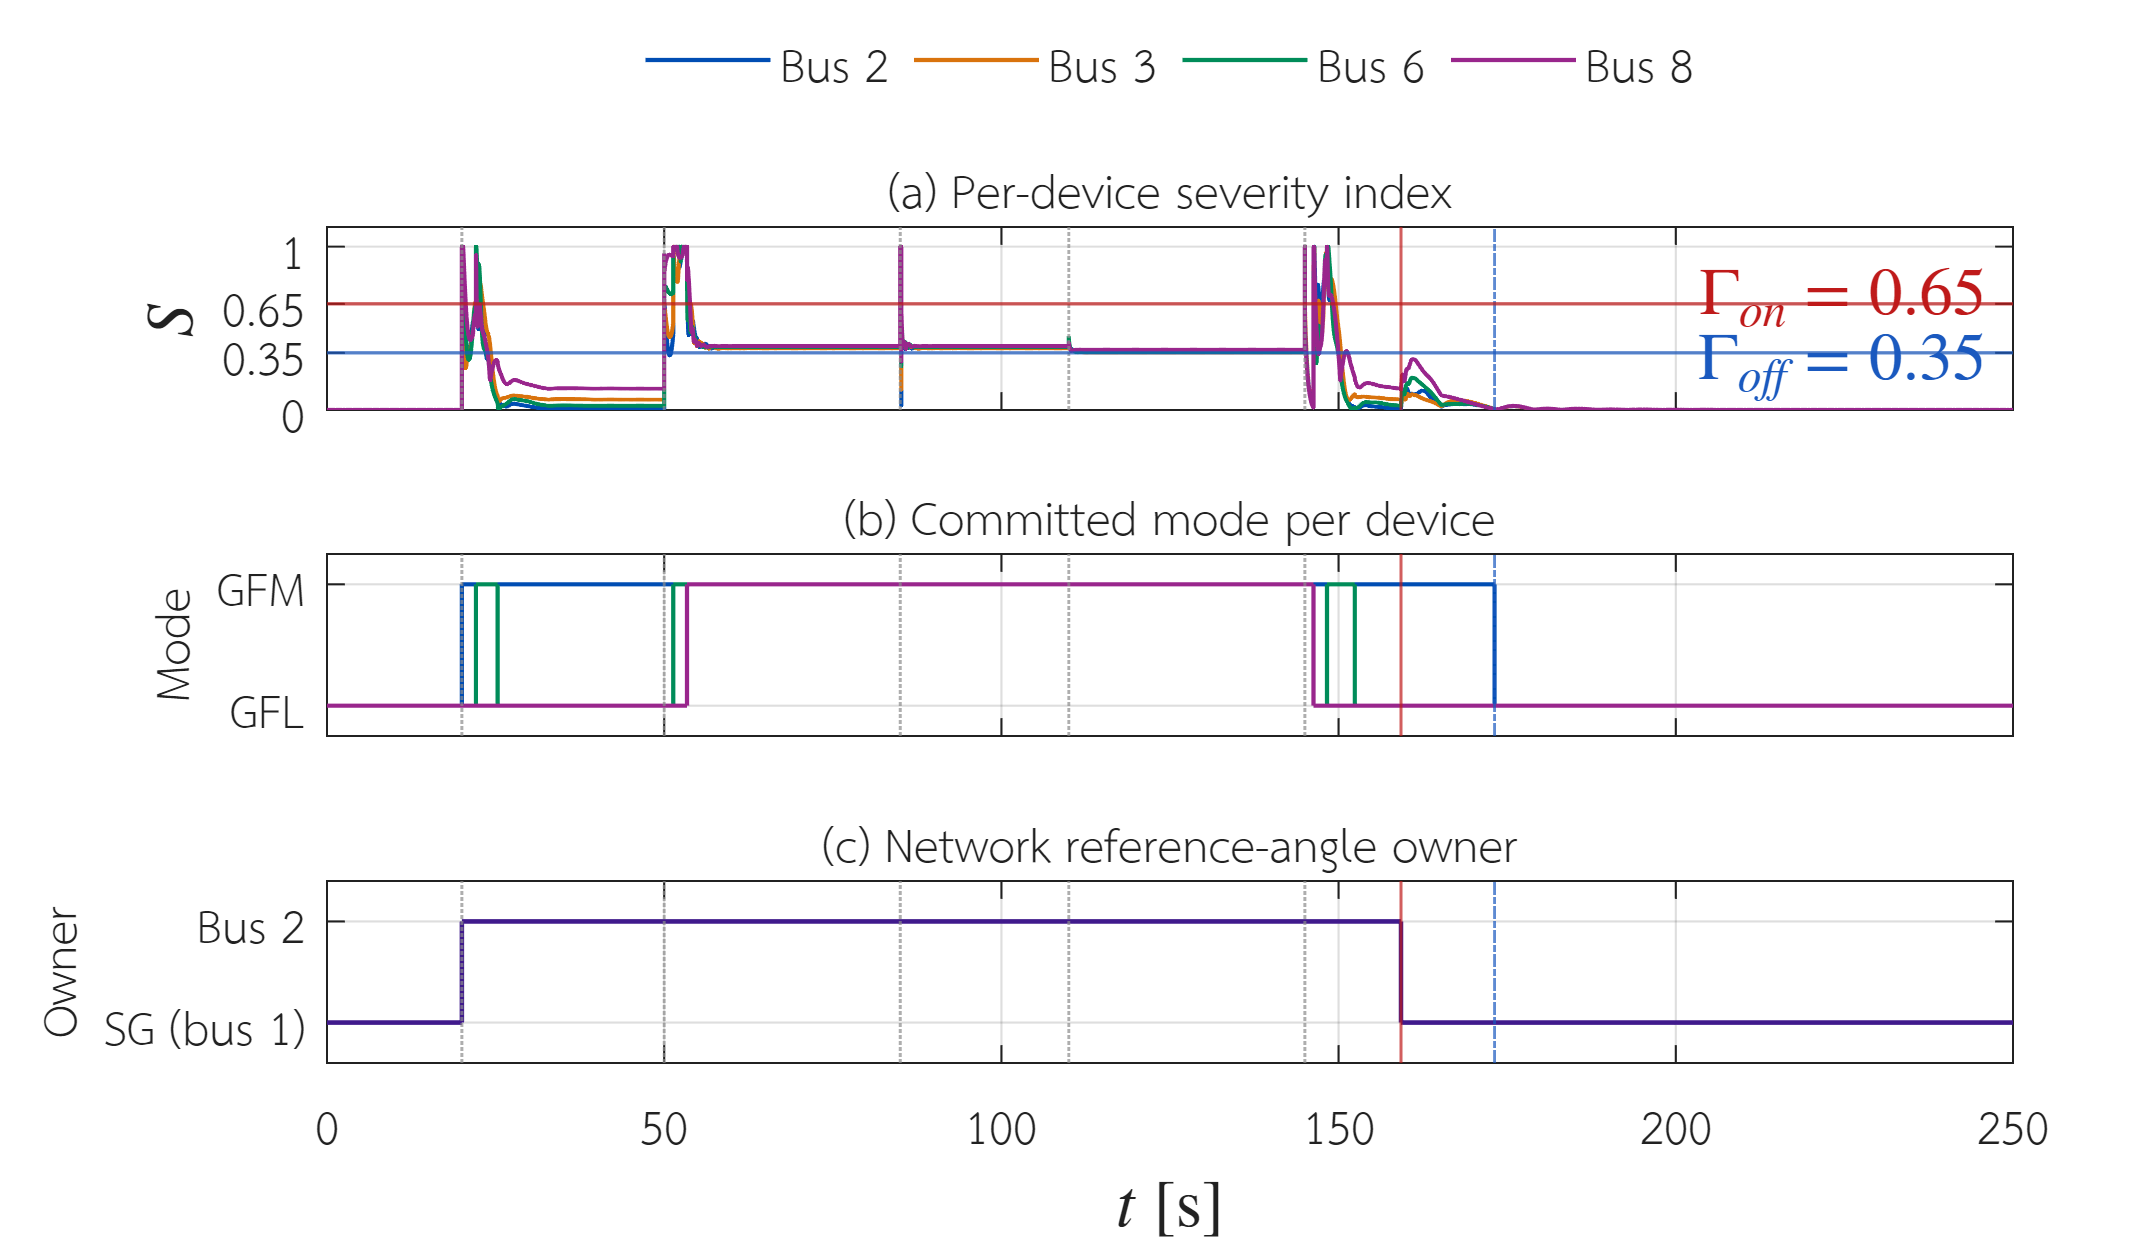
\includegraphics[width=0.94\textwidth]{fig_supervisor.png}
\caption{Severity index, สถานะ GFL/GFM และผู้ถือ reference angle ของ adaptive trajectory}
\label{fig:supervisor}
\end{figure}

\templatesubheading{11. วิธีตรวจสอบและหลักฐานที่ใช้ยืนยันแบบจำลอง}
โครงงานใช้แนวทาง ``สมการเดียวกัน--หลายการตรวจสอบ'' คือไม่สร้าง simplified model แยกขึ้นมาเพื่อทำให้ผล validation ผ่าน ตารางที่~\ref{tab:validation} สรุปสิ่งที่ตรวจและเหตุผลของแต่ละ gate โดยผลทั้งหมดในรายงานนี้อ้างเฉพาะกรณี IEEE 14-bus และแบบจำลองที่ประกอบอยู่ในกรณีดังกล่าว
\begin{table}[H]
\centering
\caption{สรุปการตรวจสอบที่ใช้กับกรอบ IEEE 14-bus}
\label{tab:validation}
\begin{tabularx}{0.98\textwidth}{@{}p{0.20\textwidth} p{0.34\textwidth} X@{}}
\toprule
ส่วนที่ตรวจ & วิธีตรวจ & เกณฑ์/หลักฐานสำคัญ \\
\midrule
Power Flow & Newton mismatch, bus/branch power balance & operating point ต้องลู่เข้าและกำลังที่คำนวณกลับจาก $V,I$ ต้องสอดคล้อง \\
DAE equilibrium & แก้ $f=0$ พร้อม KCL ทุกแถว & ไม่ตัด physical KCL ของ REF bus; state และ input ชุดนี้ถูก reuse ใน SSSA/TS \\
SSSA & linearize full-KCL DAE และจัดการ gauge ก่อน eig & physical eigenvalues finite; candidate ต้องมี damping margin ตามเกณฑ์ที่ freeze ไว้ \\
IBR model & equilibrium residual, mode ownership, frame covariance & GFM branch ไม่มี PLL; GFL PLL ต้องตอบสนองต่อ $v_q$; inactive state ต้อง hold \\
DC source & equilibrium, stable DC pair, capacitance sensitivity & $V_{dc},I_{dc}$ เป็น equilibrium ที่ dispatch และคู่ DC eigenvalue อยู่ left-half plane \\
Mode transfer & คำนวณ terminal port ก่อน/หลัง & $|I^+-I^-|\le10^{-10}$ และ $P,Q,V_{dc},I_{dc}$ ต่อเนื่องตาม contract \\
TS solver & implicit residual + rejected-step rollback & accepted residual ต่ำกว่า $10^{-8}$; rejected trial ไม่ถูกบันทึกเป็น trajectory \\
Event handling & exact event landing + right-limit solve & ไม่ให้ time step คร่อม topology/mode สองชุด \\
Supervisor & reference guard + authenticated candidate + certificate & ไม่มีช่วง energized island ที่ไร้ voltage-forming source และไม่ commit candidate ที่ nonlinear trial ไม่ผ่าน \\
Regression & fixed default เทียบ explicit fixed บน IEEE14 & $t,x,y,u$ และ event log ตรงกันแบบ bit-identical \\
\bottomrule
\end{tabularx}
\end{table}

\templatesubheading{12. เหตุการณ์ทดสอบและผล Time-Domain Simulation หลัก}
กรณีหลักจำลองเป็นเวลา 250 s เพื่อให้ครอบคลุมทั้งการสูญเสีย SG, การเปลี่ยนกำลังโหลด, fault, topology change และ restoration ดังตารางที่~\ref{tab:events}
\begin{table}[H]
\centering
\caption{ลำดับเหตุการณ์ของกรณี IEEE 14-bus}
\label{tab:events}
\begin{tabularx}{0.94\textwidth}{@{}r l X@{}}
\toprule
เวลา (s) & เหตุการณ์ & รายละเอียด \\
\midrule
20.000 & SG trip & เปิด breaker ของ SG ที่บัส 1 และเข้าสู่ช่วง islanded reference by IBR \\
50.000 & Load step & เพิ่มโหลดเพื่อทดสอบ active-power support และ droop response \\
85.000--85.150 & Fault & fault ที่บัส 9, $Z_f=0.01+j0.01$ pu แล้ว clear หลัง 0.15 s \\
110.000 & Line trip & ปลดสาย 6--13 และเปลี่ยน $Y_{net}$ ของระบบ \\
145.000 & Restore request & เริ่มกระบวนการคืน SG และตรวจ synchronism \\
159.252 & SG reclose & breaker SG ปิดสำเร็จตาม accepted event log \\
173.127 & Final mode return & IBR ตัวสุดท้ายคืนจาก GFM ไป GFL หลัง handback \\
250.000 & End & จบ simulation horizon \\
\bottomrule
\end{tabularx}
\end{table}

ผล adaptive trajectory เดินครบ 250 s มี accepted samples 3679 จุด และ rejected controller steps 161 ครั้ง การมี rejected step ไม่ใช่ความล้มเหลวของผล เพราะ step เหล่านี้ถูก rollback และลดขนาดเวลาใหม่ก่อนรับคำตอบ จุดที่สำคัญคือ largest residual ของ accepted trajectory เท่ากับ $9.9721\times10^{-9}$ ซึ่งยังต่ำกว่า $10^{-8}$ gate
\begin{table}[H]
\centering
\caption{ผลสรุปของ adaptive trajectory ล่าสุด}
\begin{tabularx}{0.94\textwidth}{@{}l l X@{}}
\toprule
Quantity & Value & ความหมาย \\
\midrule
Simulation horizon & 250.000 s & เดินครบ horizon โดยไม่ extrapolate \\
Transient voltage range & 0.036855--1.523199 pu & extrema ระหว่าง fault/switching ไม่ใช่ operating rating \\
COI frequency range & 58.839081--61.138547 Hz & extrema ของเหตุการณ์ทั้งหมด \\
Terminal COI frequency & 60.000001 Hz & กลับใกล้ nominal ที่ปลาย run \\
Terminal voltage range & 0.9667--1.0575 pu & ช่วงแรงดันที่ $t=250$ s \\
Largest accepted residual & $9.9721\times10^{-9}$ & ผ่าน $10^{-8}$ residual gate \\
SG reclose & 159.252 s, SUCCESS & $\Delta V=0.008785$ pu, $\Delta\theta=5.015^{\circ}$ \\
Final GFL return & 173.127 s & reference ownership ส่งกลับ SG แล้ว \\
Maximum simultaneous GFM & 4 & เพิ่มเป็นลำดับ ไม่ได้สั่งทั้งสี่พร้อมกัน \\
\bottomrule
\end{tabularx}
\end{table}
\begin{figure}[H]
\centering
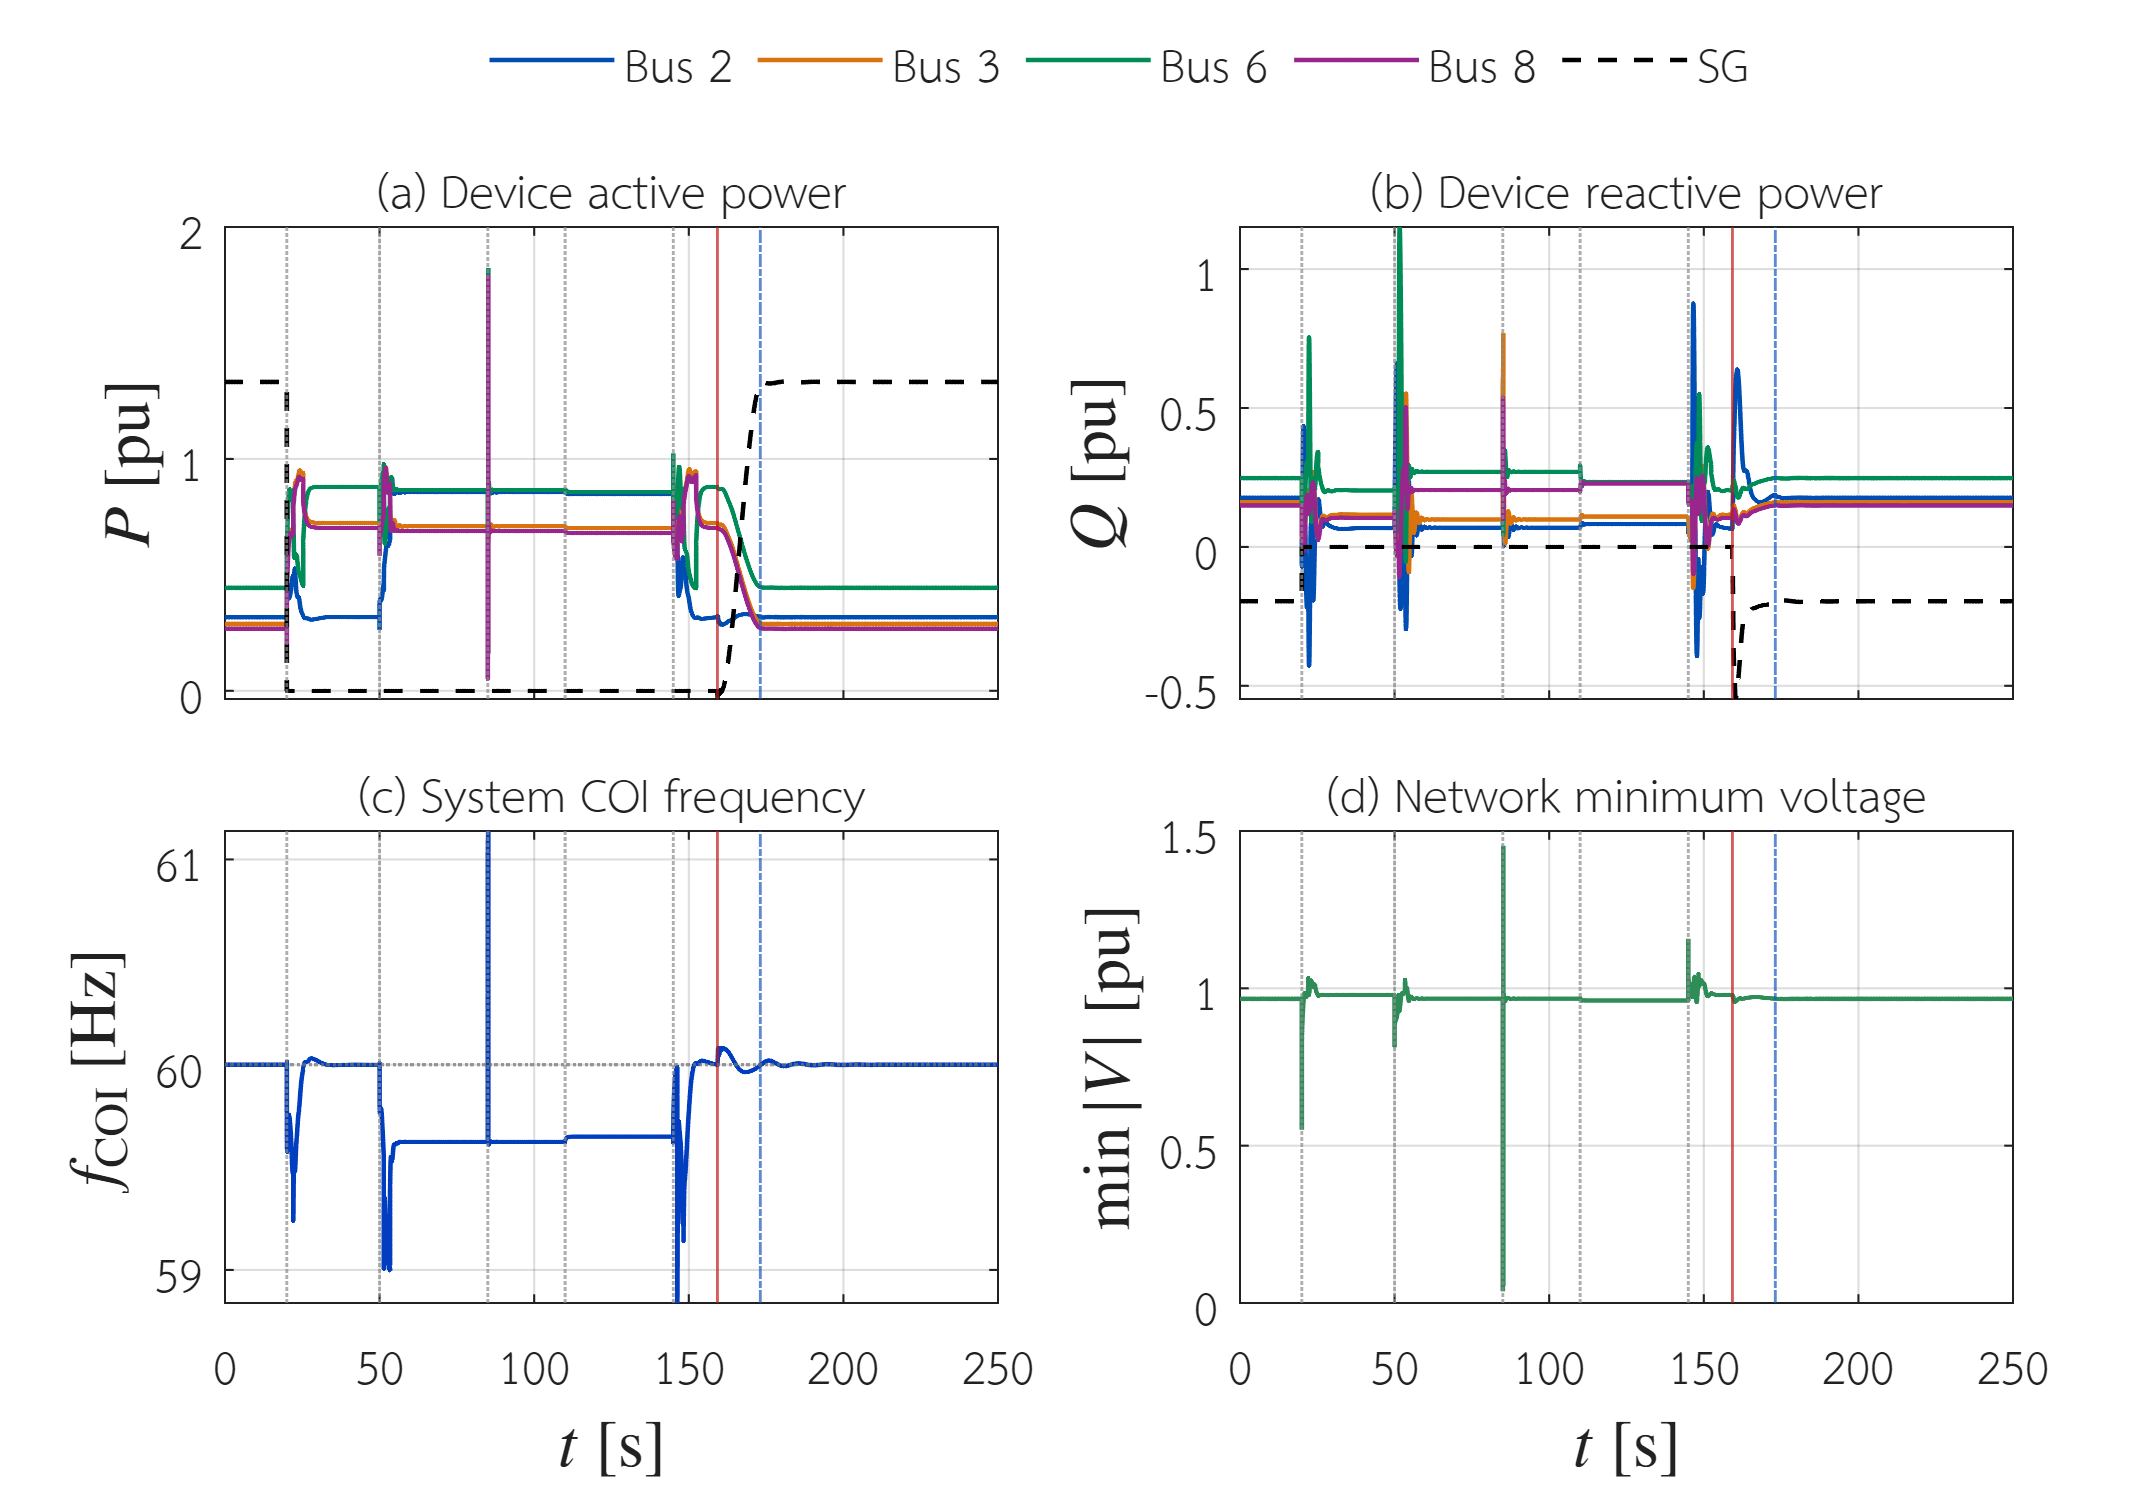
\includegraphics[width=0.96\textwidth]{fig_electrical.png}
\caption{ผลตอบสนองทางไฟฟ้าของ adaptive switching arm ตลอดลำดับเหตุการณ์}
\label{fig:electrical}
\end{figure}

จาก event log supervisor เพิ่ม GFM ที่ 22.089, 51.340, 53.379 และ 148.281 s และลด support ที่ 25.303, 146.278 และ 152.402 s ก่อนคืน IBR ตัวสุดท้ายสู่ GFL ที่ 173.127 s หลัง SG กลับมา การเพิ่ม support แบบ staged นี้เกิดจาก severity/dwell และ authenticated candidate selection ไม่ได้ผูกจำนวน GFM กับเวลารบกวนแบบ hard-coded

\templatesubheading{13. การเปรียบเทียบนโยบายและสิ่งที่สรุปได้จากผล}
เพื่อแยกผลของ ``การสลับตามสภาวะ'' ออกจากผลของ ``มี GFM อยู่เฉย ๆ'' ได้ทดลอง policy หลายแบบบน network, dispatch, event schedule และ solver เดียวกัน ผลสรุปแสดงในตารางที่~\ref{tab:policy}
\begin{table}[H]
\centering
\caption{การเปรียบเทียบนโยบายบน IEEE 14-bus เดียวกัน}
\label{tab:policy}
\begin{tabularx}{0.98\textwidth}{@{}l r l X@{}}
\toprule
นโยบาย & Horizon (s) & ผล & ข้อสังเกต \\
\midrule
Adaptive switching & 250.000 & สำเร็จ & เพิ่ม/ลด GFM ตาม severity และคืน SG สำเร็จ \\
Pinned GFM = 1 & 250.000 & สำเร็จ & อยู่ได้แต่ frequency support ต่ำกว่า adaptive หลายช่วง \\
Pinned GFM = 2 & 250.000 & สำเร็จ & ดีขึ้นจากหนึ่งตัวในบาง event แต่ไม่มีการปรับตามสภาวะ \\
Pinned GFM = 4 & 25.485 & หยุด & ผ่าน linear screen แต่ nonlinear path ไปไม่ถึง configuration อย่างเสถียรเมื่อ pin ตั้งแต่ trip \\
Locked GFL & 20.000 & ปฏิเสธ & SG trip แล้วไม่มี voltage-forming source \\
No adaptation & 250.000 & สำเร็จ & commit GFM หนึ่งตัวแล้วไม่เพิ่ม support เมื่อ disturbance รุนแรงขึ้น \\
\bottomrule
\end{tabularx}
\end{table}

\begin{figure}[H]
\centering
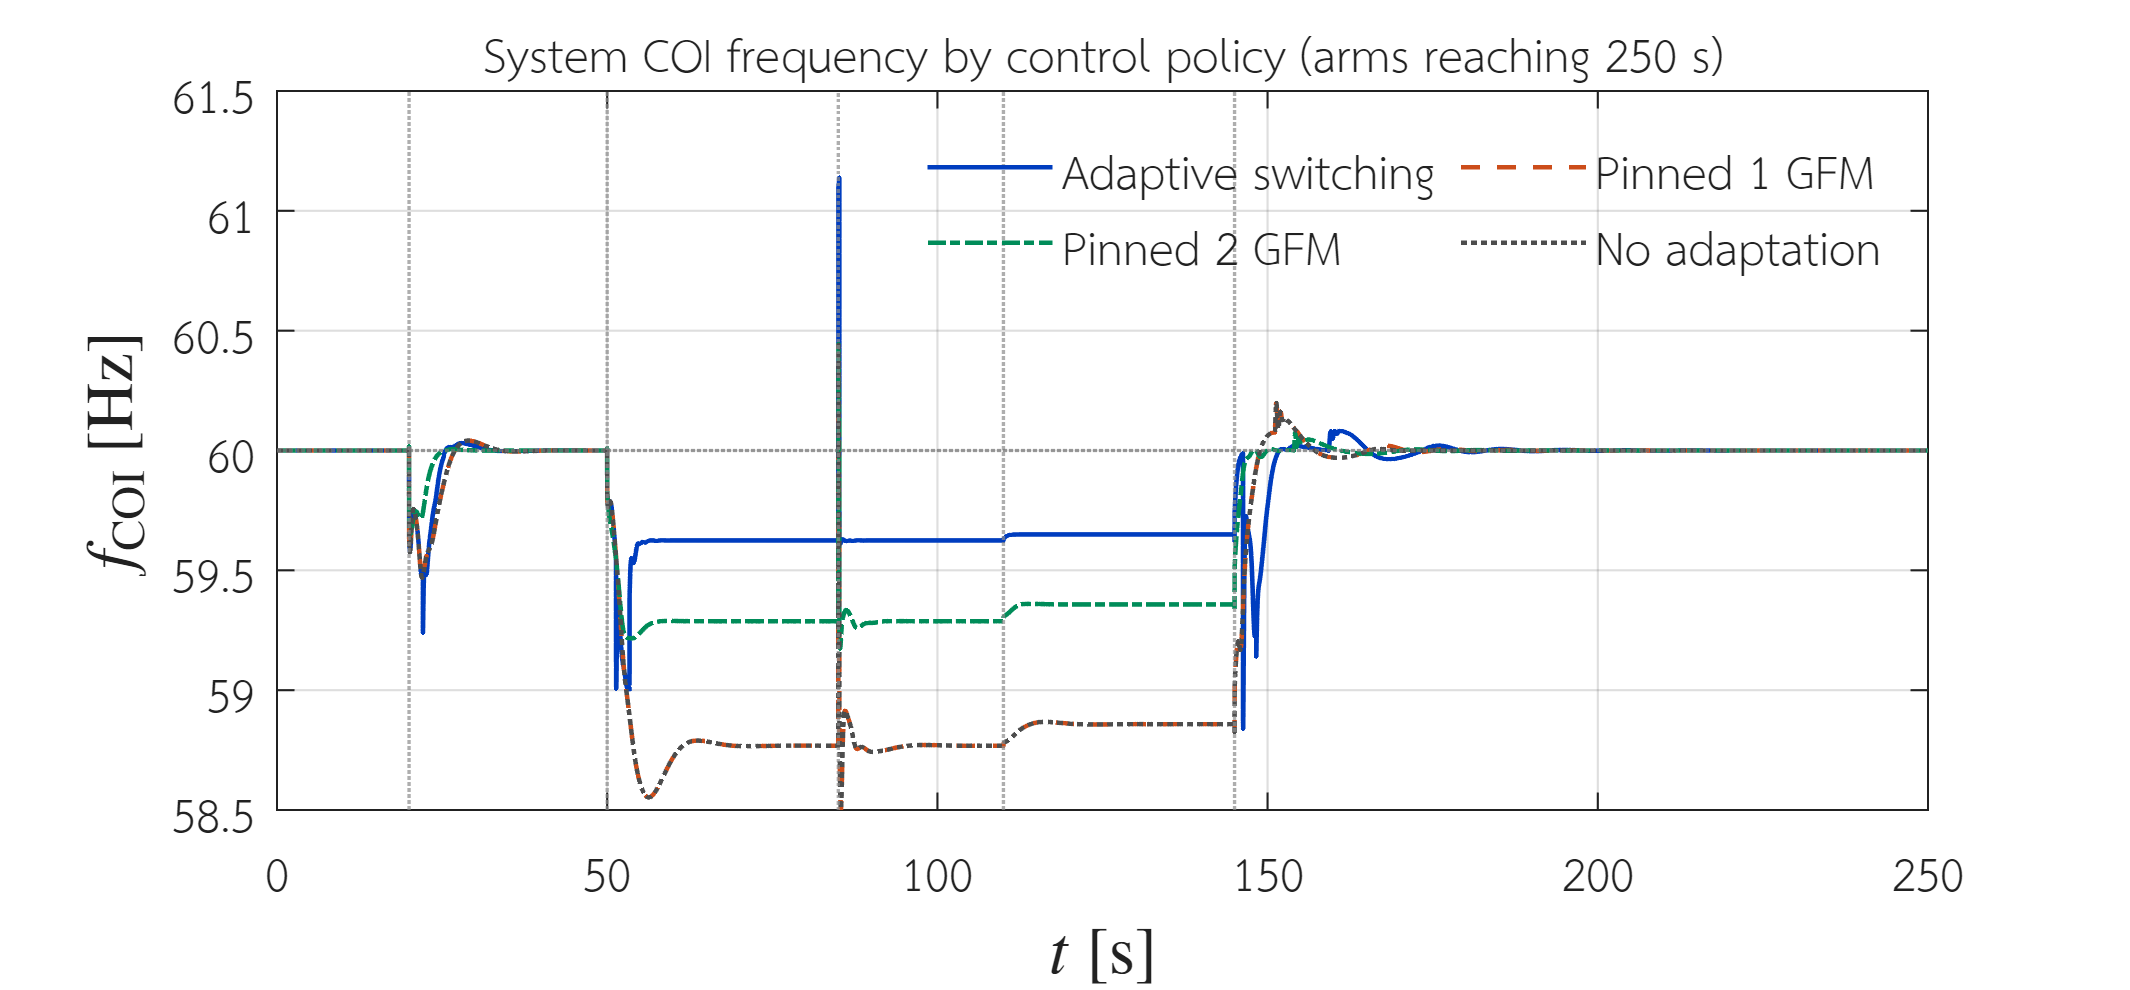
\includegraphics[width=0.94\textwidth]{fig_policy.png}
\caption{ผลเปรียบเทียบ adaptive switching กับนโยบายควบคุมอื่นภายใต้เหตุการณ์เดียวกัน}
\label{fig:policy}
\end{figure}

ผลนี้ให้ข้อสรุปสำคัญสามประการ ประการแรก หลังสูญเสีย SG ต้องมี voltage-forming source อย่างน้อยหนึ่งตัว มิฉะนั้นปัญหาไม่ใช่เพียง ``frequency แย่'' แต่เป็นระบบไม่มี reference และสมการไม่ควรถูกแก้ต่อ ประการที่สอง candidate ที่ผ่าน SSSA ไม่ได้หมายความว่าจะเดินทางจาก state ปัจจุบันไปถึง candidate นั้นได้ใน nonlinear TS ดังที่เห็นจาก pinned 4-GFM ซึ่งผ่าน linear screen แต่หยุดที่ 25.485 s ประการที่สาม adaptive policy มีประโยชน์จาก \emph{ลำดับการเปลี่ยนโหมด} ไม่ใช่เพียง final set ของ GFM เพราะระบบเพิ่ม forming support ทีละขั้นและตรวจ transition ก่อน commit

\templatesubheading{14. สรุปผลงานที่พัฒนาได้จริงในโครงงาน}
จากการดำเนินงานสามารถสรุปสิ่งที่พัฒนาและทดสอบได้ดังนี้
\begin{enumerate}
\item พัฒนา Power Flow ของ IEEE 14-bus และ mapping จาก PF ไปยัง DAE equilibrium โดยใช้ convention ของแรงดัน กระแส กำลัง และ per-unit base ชุดเดียวกัน
\item พัฒนา SSSA บน full-KCL composite DAE พร้อม Schur reduction, reference/gauge treatment และ candidate enumeration สำหรับ configuration ของ GFM
\item พัฒนา implicit-trapezoidal TS ที่รองรับ nonlinear Newton solve, adaptive step, rollback และ exact event landing
\item รวม SG และ IBR หลายตัวใน composite DAE เดียว โดยแต่ละอุปกรณ์ให้ current injection ผ่าน interface เดียวกัน
\item พัฒนา IBR 17-coordinate dual-mode ที่มี common AC/DC plant, GFL branch ที่ใช้ PLL และ GFM branch ที่ใช้ VSG โดยมี current limiting และ anti-windup
\item พัฒนา physical transfer map ระหว่าง GFL/GFM ที่รักษา terminal current, $P/Q$, $V_{dc}$ และ $I_{dc}$ ตาม tolerance ก่อน commit
\item พัฒนา automatic supervisor ที่ใช้ voltage/frequency severity, hysteresis, dwell, reference guard, equilibrium/SSSA candidate table และ nonlinear transition certificate
\item ทดสอบ end-to-end บน IEEE 14-bus ด้วย SG trip, load step, fault, line trip และ SG restoration จน adaptive trajectory เดินครบ 250 s และคืนระบบกลับสู่ all-GFL หลัง SG reclose
\end{enumerate}
\clearpage
\templateheading{ประโยชน์ที่ได้รับจากโครงงาน}
\templatesubheading{ประโยชน์ด้านวิชาการและการพัฒนาแบบจำลอง}
\begin{enumerate}
\item ได้กรอบการจำลองระบบไฟฟ้ากำลังที่ใช้สมการและ state mapping ร่วมกันตั้งแต่ PF, equilibrium, SSSA จนถึง TS ทำให้ตรวจสอบความสอดคล้องของผลได้ง่ายขึ้น
\item ได้แบบจำลอง IBR ที่สามารถสลับระหว่าง GFL และ GFM ภายใน container เดียว โดยรักษา state ทางกายภาพที่สำคัญเมื่อเปลี่ยนโหมด
\item ได้แนวทางใช้ small-signal screening ร่วมกับ nonlinear time-domain validation เพื่อหลีกเลี่ยงการสรุปผลจาก eigenvalue เพียงอย่างเดียว
\item ได้ชุดกรณีศึกษา IEEE 14-bus ที่มีเหตุการณ์หลายชนิดสำหรับใช้ทดสอบงานด้าน IBR และการเปลี่ยนโหมดในอนาคต
\end{enumerate}

\templatesubheading{ประโยชน์ด้านการประยุกต์ใช้งาน}
\begin{enumerate}
\item แนวคิด supervisor สามารถใช้เป็นพื้นฐานในการศึกษาการจัดสรรบทบาท GFM เฉพาะช่วงที่ระบบต้องการ voltage-forming support แทนการกำหนดให้ converter ทุกตัวทำงานในโหมดเดียวตลอดเวลา
\item กรอบการทำงานช่วยศึกษาการถ่ายโอนผู้ถือมุมอ้างอิงระหว่าง SG และ IBR เมื่อระบบเกิด islanding หรืออยู่ในช่วง restoration
\item ผลการเปรียบเทียบนโยบายช่วยให้เห็น trade-off ระหว่างความมั่นคงของระบบ จำนวน IBR ที่ทำหน้าที่ GFM และความซับซ้อนของการควบคุม
\end{enumerate}

\templateheading{ปัญหาและอุปสรรคที่เกิดขึ้น}
\begin{enumerate}
\item หลัง SG trip ระบบไม่สามารถแก้สมการต่อได้หากไม่มี IBR อย่างน้อยหนึ่งตัวทำหน้าที่ voltage-forming เนื่องจากไม่มีแหล่งกำหนดมุมอ้างอิงของโครงข่าย
\item การสลับ GFL/GFM ทำให้ state order และ controller states เปลี่ยนบทบาท หาก map state ไม่ถูกต้องอาจเกิด discontinuity ของกระแสและทำให้ Newton corrector ไม่ลู่เข้า
\item candidate ที่ผ่าน SSSA ไม่ได้หมายความว่าจะผ่าน nonlinear TS เสมอ ตัวอย่างคือกรณีตรึง GFM ทั้ง 4 ตัวซึ่งผ่าน linear screen แต่หยุดก่อนครบ horizon
\item การจำลองแบบ implicit และ adaptive time step ใช้เวลาคำนวณสูง โดยเฉพาะช่วง fault หรือช่วงที่ topology เปลี่ยนและต้องแก้ nonlinear equations ซ้ำหลายครั้ง
\item แบบจำลอง IBR ต้นทางให้สมการฝั่ง AC/control แต่ไม่ได้กำหนดกฎของแหล่งจ่ายฝั่ง DC ครบถ้วน หากปิดสมการด้วย ideal source จะทำให้ $V_{dc}$ แทบไม่ตอบสนองและ $C_{dc}$ หายออกจากพลวัต จึงต้องสร้าง DC-source closure ที่มีความหมายทางกายภาพและตรวจเสถียรภาพแยกต่างหาก
\end{enumerate}
\templateheading{แนวทางการแก้ไขปัญหาและอุปสรรคที่เกิดขึ้น}
\begin{enumerate}
\item กำหนด reference-owner guard ให้ระบบตรวจว่ามี SG หรือ GFM อย่างน้อยหนึ่งแหล่งก่อนเรียกตัวแก้สมการ หากไม่มีให้หยุดแบบ fail-closed แทนการฝืนคำนวณต่อ
\item ใช้ fixed superset state สำหรับ IBR และกำหนดขั้นตอน state transfer ที่ชัดเจน โดย carry plant states, initialize controller states จาก accepted operating point และตรวจ terminal-current continuity ก่อน commit
\item ใช้ SSSA เป็นเพียง screening ขั้นแรก และยืนยัน candidate ที่เลือกด้วย nonlinear TS ทุกครั้ง เพื่อไม่ให้ผลเชิงเส้นถูกตีความเกินขอบเขต
\item ใช้ implicit trapezoidal solver ร่วมกับ adaptive step control, exact event landing และ rollback ของ rejected step เพื่อลดปัญหาการลู่เข้าในช่วง disturbance รุนแรง
\item แทน ideal DC closure ด้วย Thevenin source ที่มี $R_{dc}$, state $I_{dc}$, capacitance $C_{dc}$ และ over-voltage chopper จากนั้นตรวจ equilibrium, eigenvalue ของ DC pair, ขอบเขต constant-power load และ sensitivity ต่อ $C_{dc}$ ก่อนนำไปใช้กับ IEEE 14-bus
\end{enumerate}

\clearpage
\templateheading{โครงงานที่คาดว่าจะดำเนินการต่อไป}
\begin{enumerate}
\item ขยายจาก balanced RMS model ไปสู่ unbalanced network และ electromagnetic transient (EMT) เพื่อศึกษาพฤติกรรม converter และ protection ในช่วงเวลาที่เร็วขึ้น
\item เพิ่มแบบจำลอง protection, current limiting, fault ride-through และข้อกำหนด grid code เพื่อให้กรณีศึกษาสะท้อนข้อจำกัดของอุปกรณ์จริงมากขึ้น
\item ทดสอบกรอบการเลือก GFM บนระบบขนาดใหญ่กว่า IEEE 14-bus และกรณีที่มี IBR จำนวนมาก เพื่อประเมิน scalability ของ candidate selection และ supervisor
\item พัฒนาเกณฑ์เลือก candidate ให้พิจารณาทั้ง damping, voltage support, converter loading, energy reserve และต้นทุนการสลับโหมดร่วมกัน
\item เชื่อมต่อแบบจำลองกับ hardware-in-the-loop หรือ controller prototype เพื่อทดสอบการเปลี่ยนโหมดและ handback ภายใต้ข้อจำกัดของระบบควบคุมจริง
\end{enumerate}

\end{document}
